\documentclass[conference]{IEEEtran}
\IEEEoverridecommandlockouts
%Template version as of 6/27/2024

\usepackage{cite}
\usepackage{amsmath,amssymb,amsfonts}
\usepackage{algorithmic}
\usepackage{graphicx}
\usepackage{textcomp}
\usepackage{xcolor}
\usepackage{float}
\usepackage{listings}
\usepackage{booktabs}
\usepackage{multirow}
\usepackage[spanish]{babel}
\usepackage[utf8]{inputenc}
\graphicspath{{../figures/}}
\def\BibTeX{{\rm B\kern-.05em{\sc i\kern-.025em b}\kern-.08em
    T\kern-.1667em\lower.7ex\hbox{E}\kern-.125emX}}

\lstset{
    basicstyle=\ttfamily\footnotesize,
    breaklines=true,
    frame=single,
    numbers=none,
    numberstyle=\tiny,
    captionpos=b
}

\begin{document}

\makeatletter
\newcommand{\linebreakand}{%
    \end{@IEEEauthorhalign}
    \hfill\mbox{}\par
    \mbox{}\hfill\begin{@IEEEauthorhalign}
}
\makeatother

\title{MicroPatosMania: Implementación de un Sistema Multijugador de Minijuegos Competitivos sobre Arquitectura P2P}

\author{\IEEEauthorblockN{1\textsuperscript{er} Mariel Alisson Jara Mamani}
    \IEEEauthorblockA{\textit{Universidad Nacional de San Agustín de Arequipa} \\
        Arequipa, Perú \\
        mjarama@unsa.edu.pe}
    \and
    \IEEEauthorblockN{2\textsuperscript{do} Christian Raul Mestas Zegarra}
    \IEEEauthorblockA{\textit{Universidad Nacional de San Agustín de Arequipa} \\
        Arequipa, Perú \\
        cmestasz@unsa.edu.pe}
}

\maketitle

\begin{abstract}
    Este trabajo presenta el desarrollo de MicroPatosMania, una plataforma multijugador de minijuegos competitivos. Dada la ausencia de una infraestructura centralizada, el sistema implementa una arquitectura lógica cliente-servidor construida sobre una red peer-to-peer (P2P), donde un nodo actúa como autoridad (Listen Server). El sistema, desarrollado en Java utilizando libGDX para renderizado y KryoNet para comunicación, integra cuatro minijuegos en un torneo por rondas. Se aplican patrones de diseño como Factory, Singleton, Strategy y Observer para garantizar extensibilidad. La plataforma soporta sesiones de 2 a 6 jugadores en redes locales, gestionando la sincronización de estado y la consistencia del juego mediante la autoridad del nodo anfitrión.
\end{abstract}

\begin{IEEEkeywords}
    arquitectura P2P, cliente-servidor, desarrollo de videojuegos, patrones de diseño, libGDX, networking multijugador, sincronización
\end{IEEEkeywords}

\section{Introducción}

Los videojuegos multijugador en redes de área local (LAN) presentan desafíos particulares en la sincronización de estado y la latencia \cite{gregory2018game}. A diferencia de los sistemas con servidores dedicados en la nube, las implementaciones LAN a menudo requieren que los dispositivos de los propios usuarios gestionen la lógica de la red.

El presente trabajo documenta el desarrollo de MicroPatosMania, una plataforma de minijuegos competitivos. Para resolver la gestión del estado compartido sin un servidor central externo, el sistema implementa una arquitectura cliente-servidor sobre una topología P2P. En este modelo, uno de los pares (peers) asume el rol de servidor autoritativo o anfitrión, manteniendo el estado canónico del juego, mientras que actúa simultáneamente como cliente local. Esta decisión permite una experiencia consistente y evita manipulaciones por parte de clientes no autoritativos, aunque introduce una dependencia crítica sobre el nodo anfitrión.

El proyecto tiene como objetivo el aprendizaje de arquitecturas de red en tiempo real y la aplicación de patrones de diseño (Factory, Singleton, Strategy, Observer) en un entorno distribuido. La plataforma integra minijuegos de recolección, combate y supervivencia en un torneo eliminatorio. La implementación utiliza libGDX \cite{libgdx} para el motor gráfico y KryoNet \cite{kryonet} para la comunicación TCP/UDP.

\section{Fundamentos y Herramientas}

\subsection{Arquitecturas de red y Sincronización}
La comunicación en videojuegos suele oscilar entre modelos peer-to-peer (P2P) puros, donde todos los clientes se comunican entre sí, y arquitecturas cliente-servidor. En entornos sin infraestructura dedicada, se adopta frecuentemente un modelo híbrido: una topología física P2P donde lógicamente un nodo actúa como servidor (Listen Server) \cite{fiedler2010networking}. Esto centraliza la autoridad del estado en un jugador, simplificando la sincronización frente a modelos de "lockstep" o P2P puro, pero aumentando la carga en la máquina del anfitrión.

La sincronización en estos sistemas distribuidos utiliza técnicas como la replicación delta, transmitiendo solo los cambios de estado para optimizar el ancho de banda frente a la replicación completa \cite{manninen2004rich}.

\subsection{Patrones de Diseño}
El sistema basa su extensibilidad en patrones clásicos \cite{gamma1995design}: Factory para la creación de entidades sin acoplamiento a clases concretas; Singleton para la gestión global de recursos y conexiones; Strategy para intercambiar la lógica de los distintos minijuegos; y Observer para desacoplar el procesamiento de eventos de red de la lógica de juego.

\subsection{Herramientas de Desarrollo}
El proyecto se implementó en Java 21, utilizando LibGDX 1.12.1 como framework central para el ciclo de vida de renderizado y gestión de assets. Para la red, se empleó KryoNet 2.22.1, que facilita la serialización eficiente de objetos Java sobre TCP y UDP. La gestión del proyecto se apoyó en Gradle para dependencias, Doxygen para documentación, y Nix para garantizar un entorno de desarrollo reproducible.

\begin{figure*}[t]
    \centering
    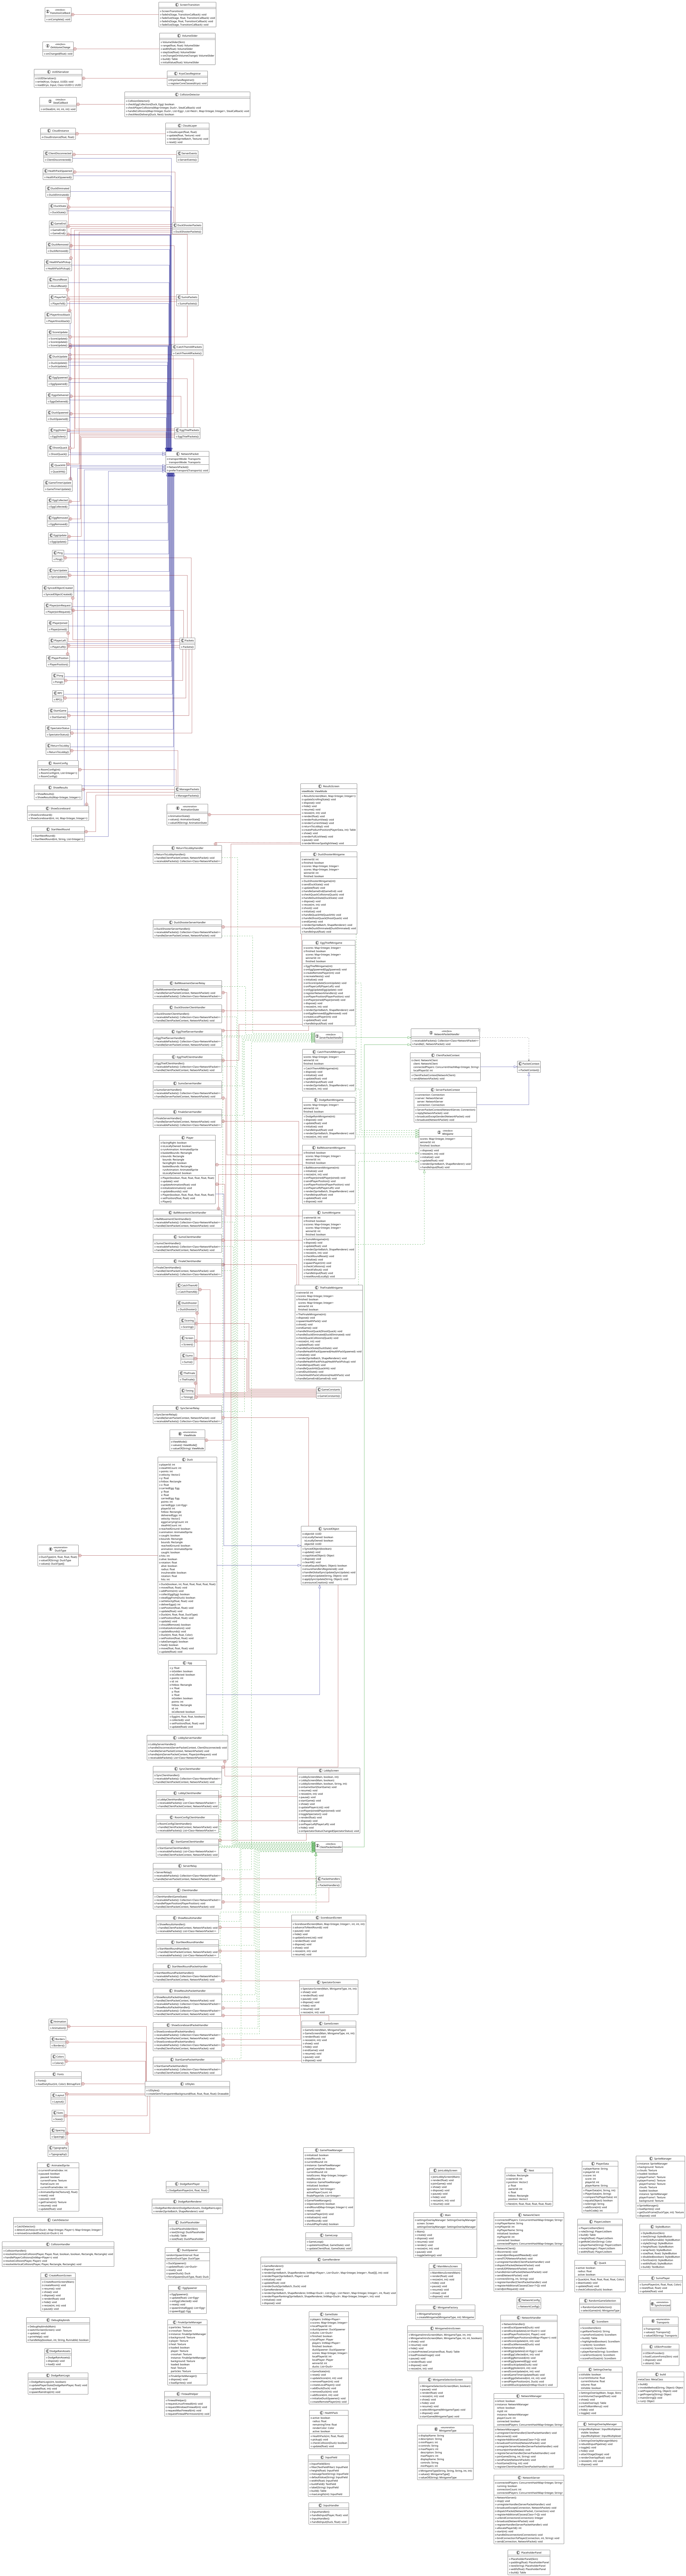
\includegraphics[width=0.265\textwidth]{architecture_uml.png}
    \caption{Diagrama UML simplificado de la arquitectura del sistema MicroPatosMania.}
    \label{fig:architecture_uml}
\end{figure*}

\section{Arquitectura del sistema}

Esta sección detalla el diseño de MicroPatosMania, enfocándose en cómo se implementa la lógica cliente-servidor sobre la estructura P2P.

\subsection{Modelo de Red P2P Autoritativo}

Debido a la inexistencia de un servidor central dedicado, MicroPatosMania opera sobre una red P2P donde la arquitectura lógica es de tipo Listen Server. Un jugador inicia la sesión actuando como Host; su instancia de juego ejecuta tanto la lógica de servidor (NetworkServer) como la de cliente local. Los demás jugadores se conectan directamente a la IP del Host actuando como clientes remotos.

El NetworkManager (Singleton) abstrae esta complejidad. Proporciona métodos unificados para el envío de paquetes, diferenciando internamente si el destinatario es un cliente remoto o el propio proceso local. El servidor mantiene un mapeo de conexiones y utiliza UUIDs de correlación para gestionar la identidad de los jugadores durante el handshake inicial, resolviendo conflictos de asignación en redes con latencia.

La comunicación utiliza KryoNet, empleando TCP para eventos críticos (inicio de ronda, eliminación) y UDP para actualizaciones de posición de alta frecuencia. Los paquetes se definen mediante clases que heredan de una base común, especificando su protocolo de transporte preferido.

\subsection{Sincronización de Estado}

Se implementó un sistema de sincronización automática mediante la clase SyncedObject y anotaciones. Los objetos del juego heredan de esta clase y marcan sus campos críticos (posición, velocidad) con @Synced. El sistema detecta cambios en estos campos y genera paquetes de actualización delta automáticamente.

\begin{lstlisting}[caption={Estructura base para objetos sincronizados.},label={lst:synced}]
public class Player extends SyncedObject {
    @Synced public float x, y;
    @Synced public float velocityX, velocityY;
    public int playerId;
    
    public Player(int playerId, int ownerId) {
        super(UUID.randomUUID(), ownerId);
        this.playerId = playerId;
    }
}
\end{lstlisting}

Solo el propietario del objeto (el Host para la mayoría de entidades, o el cliente específico para su propio avatar) tiene autoridad para modificarlo. Estos cambios se propagan al servidor (si el origen es un cliente) y luego se difunden al resto de la red, garantizando coherencia.

\subsection{Gestión de Minijuegos y Torneo}

El núcleo del juego utiliza el patrón Strategy a través de la interfaz Minigame. Esto permite al gestor de flujo (GameFlowManager) ejecutar cualquier minijuego sin conocer su implementación interna.

\begin{lstlisting}[caption={Interfaz Minigame.},label={lst:minigame}]
public interface Minigame {
    void create();
    void render(float delta);
    void handleInput();
    void dispose();
    void registerClientHandlers(NetworkClient c);
    void registerServerHandlers(NetworkServer s);
}
\end{lstlisting}

La instanciación se maneja mediante una Factory que retorna la implementación concreta según el tipo de juego seleccionado. Cada minijuego es autónomo: gestiona sus propios assets, define sus paquetes de red específicos y registra sus handlers mediante el patrón Observer al iniciarse.

El torneo sigue una secuencia de rondas configurables. El GameFlowManager acumula puntuaciones y decide la transición entre pantallas (Lobby, Explicación, Juego, Resultados). La selección de minijuegos intermedios es aleatoria, mientras que la ronda final ("The Finale") se reserva para el cierre, filtrando a los jugadores (top 30\%) y pasando al resto a modo espectador.

\subsection{Manejo de Entrada y Autoridad}

El manejo de entrada refuerza el modelo de autoridad del servidor. Los clientes capturan el input local y lo envían inmediatamente al Host. El Host valida la acción según el estado actual del juego, la aplica y difunde el resultado. Para mejorar la respuesta local, se utiliza una predicción limitada en el cliente, aunque el estado del servidor siempre prevalece en caso de discrepancia (reconciliación).

\section{Minijuegos Implementados}

El sistema integra cuatro minijuegos que demuestran diferentes aspectos de la sincronización en red.

\subsection{Catch Them All}
Juego de recolección donde los jugadores atrapan objetos que caen. El Host (servidor) controla la generación procedural de patos y la detección de colisiones. La sincronización es crítica aquí para asegurar que todos los clientes vean el mismo tipo de pato y posición. Cuando el servidor detecta una captura, difunde un paquete de evento que actualiza la puntuación y elimina la entidad en todos los clientes.

\begin{figure}[htbp]
    \centering
    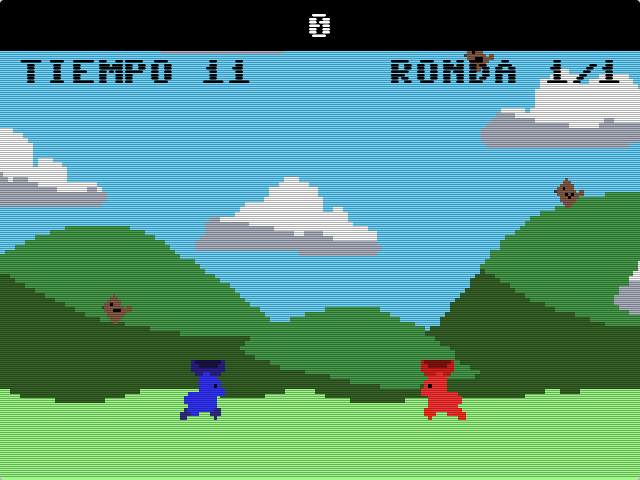
\includegraphics[width=0.45\textwidth]{catch_them_all.png}
    \caption{Catch Them All: competencia de recolección.}
    \label{fig:catch_them_all}
\end{figure}

\subsection{Pond Push (Sumo)}
Combate físico en una plataforma circular. Implementa física de colisiones y cálculo de vectores de empuje. El servidor verifica en cada frame si un jugador ha salido del radio permitido. La transmisión de posiciones vía UDP es fundamental para mantener la fluidez del combate cuerpo a cuerpo.

\begin{figure}[htbp]
    \centering
    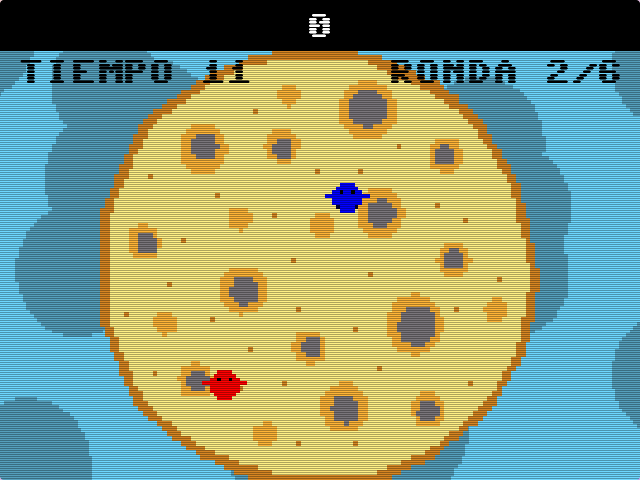
\includegraphics[width=0.45\textwidth]{pond_push.png}
    \caption{Pond Push: combate físico en plataforma.}
    \label{fig:pond_push}
\end{figure}

\subsection{Dodge Rain}
Minijuego de supervivencia. Los jugadores esquivan obstáculos con diferentes efectos (daño, ralentización). El servidor gestiona la dificultad progresiva, aumentando la frecuencia y velocidad de caída de los objetos. La sincronización asegura que los estados alterados (como la reducción de velocidad) se reflejen consistentemente.

\begin{figure}[htbp]
    \centering
    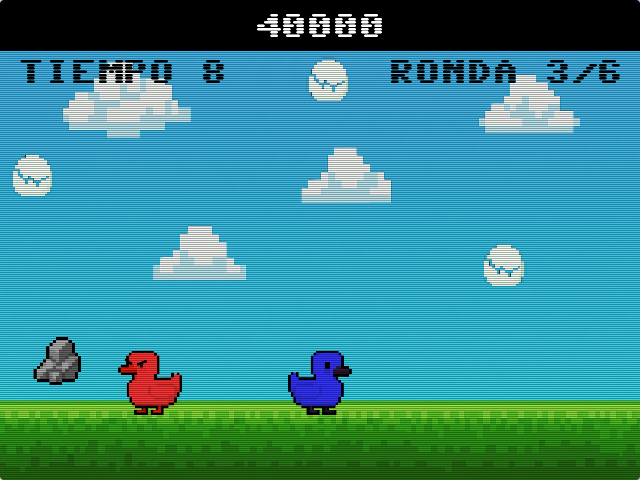
\includegraphics[width=0.45\textwidth]{dodge_rain.png}
    \caption{Dodge Rain: supervivencia ante obstáculos.}
    \label{fig:dodge_rain}
\end{figure}

\subsection{The Finale}
Batalla final con mecánicas de disparo. Incluye gestión de proyectiles, salud y frames de invulnerabilidad. Solo los finalistas participan; el resto recibe datos solo para renderizado (modo espectador). La detección de impacto es autoritativa en el servidor para evitar trampas.

\begin{figure}[htbp]
    \centering
    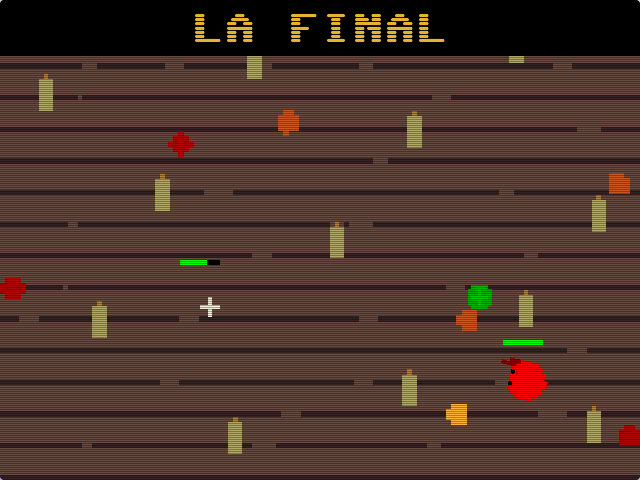
\includegraphics[width=0.45\textwidth]{the_finale.png}
    \caption{The Finale: batalla de eliminación directa.}
    \label{fig:the_finale}
\end{figure}

\section{Detalles de Implementación Avanzados}

\subsection{Sistema de Sincronización mediante Reflexión}

Uno de los componentes técnicamente más sofisticados del sistema es el mecanismo de sincronización basado en reflexión. La clase SyncedObject utiliza la API de reflexión de Java para inspeccionar los campos de las entidades del juego en tiempo de ejecución, detectando automáticamente aquellos marcados con la anotación @Synchronized.

El proceso funciona en tres fases: (1) Durante la construcción del objeto, se cachean todos los campos anotados y sus valores iniciales mediante reflection API; (2) En cada frame, el método update() compara los valores actuales con los cacheados usando Field.get() para detectar cambios; (3) Cuando se detecta una modificación, se genera un paquete SyncUpdate con el UUID del objeto, el nombre del campo y el nuevo valor, que se envía selectivamente vía UDP.

Este diseño reduce drásticamente el acoplamiento entre la lógica del juego y la capa de red. Los desarrolladores simplemente anotan los campos críticos sin necesidad de implementar código de serialización manual. El sistema maneja automáticamente la propagación de cambios mediante handlers de tipo Observer que interceptan los paquetes SyncUpdate en el servidor y los retransmiten al resto de clientes.

La implementación utiliza un mapa estático ConcurrentHashMap que asocia cada UUID con su instancia de SyncedObject, permitiendo que el handler global enrute las actualizaciones al objeto correcto. Para evitar actualizaciones circulares, solo los objetos marcados como isLocallyOwned=true pueden modificar sus propios campos; las instancias remotas son de solo lectura.

\subsection{Gestión de Recursos y Optimizaciones}

LibGDX requiere una gestión explícita de memoria debido a su uso de recursos nativos OpenGL. El sistema implementa el patrón Disposable de forma estricta: cada pantalla (Screen) y cada minijuego llama a dispose() sobre sus assets (Texturas, Fonts, Stages) al ser desechados. Esto evita memory leaks críticos que en pruebas tempranas causaban degradación del rendimiento tras varias partidas consecutivas.

Para reducir los tiempos de carga, se utiliza un AssetManager centralizado que precarga sprites compartidos durante la pantalla de lobby. Los minijuegos individuales solo cargan sus assets específicos de forma lazy, descargándolos inmediatamente después de terminar la ronda.

La serialización de paquetes se optimiza mediante el registro explícito de clases en Kryo. KryoNet permite asignar IDs numéricos a las clases más utilizadas (SyncUpdate, PlayerPosition), reduciendo el overhead de metadatos en cada transmisión UDP. Esto es particularmente importante para las actualizaciones de posición que se envían a 30Hz.

\subsection{Seguridad y Validación}

Aunque el sistema no implementa criptografía (dado que opera en redes LAN confiables), incluye validaciones básicas del lado del servidor. El Host verifica todas las acciones críticas: detección de colisiones en Catch Them All, cálculo de daño en The Finale, y expulsión de jugadores en Pond Push son procesados exclusivamente por el servidor.

Los clientes envían solo inputs (teclas presionadas, dirección de movimiento), nunca estados finales como "he atrapado un pato" o "he eliminado al jugador X". El servidor recalcula estas acciones basándose en su propia simulación autoritativa. Esto previene la mayoría de los exploits básicos, aunque un atacante con conocimiento del protocolo podría inyectar paquetes de input falsos (por ejemplo, posición imposible).

Para mitigar latencia en la experiencia del usuario, los clientes implementan una predicción local limitada: cuando el jugador presiona una tecla, su avatar se mueve inmediatamente en el cliente sin esperar la confirmación del servidor. Si el servidor detecta discrepancias (por ejemplo, un intento de atravesar una pared), envía una corrección de estado que el cliente acepta incondicionalmente, provocando un "teleport" correctivo visible.

\section{Validación y Resultados}

\subsection{Funcionalidad de Red}
Las pruebas en redes LAN (latencia $<$5ms) validaron la arquitectura Listen Server. El descubrimiento de servidor y la conexión mediante IP funcionan correctamente. La asignación de identidad mediante UUIDs solucionó problemas de concurrencia en el login. El uso híbrido de TCP/UDP demostró ser efectivo: la posición de los jugadores es fluida, y los eventos de juego (puntuación, muerte) son consistentes. Sin embargo, en pruebas con latencia simulada ($>$100ms), la falta de interpolación compleja del lado del cliente provoca saltos visibles, limitando el sistema idealmente a entornos LAN.

\subsection{Flujo de Juego}
El sistema de torneo gestiona adecuadamente las transiciones y la acumulación de puntaje. La lógica de eliminación en la fase final y el modo espectador operan según lo diseñado. Se identificó una limitación en la limpieza de recursos de red si se interrumpe el juego abruptamente desde el menú de pausa, requiriendo reinicio.

\subsection{Pruebas de Estrés y Escalabilidad}
Se realizaron pruebas con el máximo de jugadores soportados (6) ejecutando múltiples rondas consecutivas. El sistema mantuvo una latencia promedio de 3ms en LAN y el consumo de ancho de banda se estabilizó en aproximadamente 15-20 KB/s por cliente durante minijuegos de alta actividad (The Finale). La memoria se mantuvo estable en 120-150 MB por instancia gracias a la gestión disciplinada de assets.

\subsection{Limitaciones}
La arquitectura P2P/Listen Server presenta un punto único de fallo: si el Host se desconecta, la sesión termina para todos, ya que no se implementó migración de host. Además, la seguridad es básica; el servidor valida acciones pero no detecta inyecciones de paquetes modificados complejos.

\section{Conclusiones}

El desarrollo de MicroPatosMania confirma la viabilidad de implementar sistemas multijugador robustos sobre arquitecturas P2P utilizando un modelo de Listen Server. El uso de patrones de diseño como Strategy y Factory fue crucial para manejar la complejidad de múltiples modos de juego sin duplicación de código.

La arquitectura basada en KryoNet permitió abstraer la complejidad del transporte, aunque la dependencia de un nodo jugador como servidor limita la escalabilidad y expone la partida a la calidad de conexión del anfitrión. El trabajo futuro debería priorizar la implementación de interpolación y predicción del lado del cliente para mitigar la latencia, así como mecanismos de migración de host para aumentar la resiliencia del sistema distribuido.

\bibliographystyle{IEEEtran}
\bibliography{refs}

\end{document}